%  LaTeX support: latex@mdpi.com
%  In case you need support, please attach all files that are necessary for compiling as well as the log file, and specify the details of your LaTeX setup (which operating system and LaTeX version / tools you are using).

%=================================================================
\documentclass[Agronomy,article,submit,moreauthors,pdftex]{mdpi}

% If you would like to post an early version of this manuscript as a preprint, you may use preprint as the journal and change 'submit' to 'accept'. The document class line would be, e.g., \documentclass[preprints,article,accept,moreauthors,pdftex]{mdpi}. This is especially recommended for submission to arXiv, where line numbers should be removed before posting. For preprints.org, the editorial staff will make this change immediately prior to posting.

%% Some pieces required from the pandoc template
\setlist[itemize]{leftmargin=*,labelsep=5.8mm}
\setlist[enumerate]{leftmargin=*,labelsep=4.9mm}


%--------------------
% Class Options:
%--------------------
%----------
% journal
%----------
% Choose between the following MDPI journals:
% acoustics, actuators, addictions, admsci, aerospace, agriculture, agriengineering, agronomy, algorithms, animals, antibiotics, antibodies, antioxidants, applsci, arts, asc, asi, atmosphere, atoms, axioms, batteries, bdcc, behavsci , beverages, bioengineering, biology, biomedicines, biomimetics, biomolecules, biosensors, brainsci , buildings, cancers, carbon , catalysts, cells, ceramics, challenges, chemengineering, chemistry, chemosensors, children, cleantechnol, climate, clockssleep, cmd, coatings, colloids, computation, computers, condensedmatter, cosmetics, cryptography, crystals, dairy, data, dentistry, designs , diagnostics, diseases, diversity, drones, econometrics, economies, education, electrochem, electronics, energies, entropy, environments, epigenomes, est, fermentation, fibers, fire, fishes, fluids, foods, forecasting, forests, fractalfract, futureinternet, futurephys, galaxies, games, gastrointestdisord, gels, genealogy, genes, geohazards, geosciences, geriatrics, hazardousmatters, healthcare, heritage, highthroughput, horticulturae, humanities, hydrology, ijerph, ijfs, ijgi, ijms, ijns, ijtpp, informatics, information, infrastructures, inorganics, insects, instruments, inventions, iot, j, jcdd, jcm, jcp, jcs, jdb, jfb, jfmk, jimaging, jintelligence, jlpea, jmmp, jmse, jnt, jof, joitmc, jpm, jrfm, jsan, land, languages, laws, life, literature, logistics, lubricants, machines, magnetochemistry, make, marinedrugs, materials, mathematics, mca, medicina, medicines, medsci, membranes, metabolites, metals, microarrays, micromachines, microorganisms, minerals, modelling, molbank, molecules, mps, mti, nanomaterials, ncrna, neuroglia, nitrogen, notspecified, nutrients, ohbm, particles, pathogens, pharmaceuticals, pharmaceutics, pharmacy, philosophies, photonics, physics, plants, plasma, polymers, polysaccharides, preprints , proceedings, processes, proteomes, psych, publications, quantumrep, quaternary, qubs, reactions, recycling, religions, remotesensing, reports, resources, risks, robotics, safety, sci, scipharm, sensors, separations, sexes, signals, sinusitis, smartcities, sna, societies, socsci, soilsystems, sports, standards, stats, surfaces, surgeries, sustainability, symmetry, systems, technologies, test, toxics, toxins, tropicalmed, universe, urbansci, vaccines, vehicles, vetsci, vibration, viruses, vision, water, wem, wevj

%---------
% article
%---------
% The default type of manuscript is "article", but can be replaced by:
% abstract, addendum, article, benchmark, book, bookreview, briefreport, casereport, changes, comment, commentary, communication, conceptpaper, conferenceproceedings, correction, conferencereport, expressionofconcern, extendedabstract, meetingreport, creative, datadescriptor, discussion, editorial, essay, erratum, hypothesis, interestingimages, letter, meetingreport, newbookreceived, obituary, opinion, projectreport, reply, retraction, review, perspective, protocol, shortnote, supfile, technicalnote, viewpoint
% supfile = supplementary materials

%----------
% submit
%----------
% The class option "submit" will be changed to "accept" by the Editorial Office when the paper is accepted. This will only make changes to the frontpage (e.g., the logo of the journal will get visible), the headings, and the copyright information. Also, line numbering will be removed. Journal info and pagination for accepted papers will also be assigned by the Editorial Office.

%------------------
% moreauthors
%------------------
% If there is only one author the class option oneauthor should be used. Otherwise use the class option moreauthors.

%---------
% pdftex
%---------
% The option pdftex is for use with pdfLaTeX. If eps figures are used, remove the option pdftex and use LaTeX and dvi2pdf.

%=================================================================
\firstpage{1}
\makeatletter
\setcounter{page}{\@firstpage}
\makeatother
\pubvolume{xx}
\issuenum{1}
\articlenumber{5}
\pubyear{2019}
\copyrightyear{2019}
%\externaleditor{Academic Editor: name}
\history{Received: date; Accepted: date; Published: date}
\updates{yes} % If there is an update available, un-comment this line

%% MDPI internal command: uncomment if new journal that already uses continuous page numbers
%\continuouspages{yes}

%------------------------------------------------------------------
% The following line should be uncommented if the LaTeX file is uploaded to arXiv.org
%\pdfoutput=1

%=================================================================
% Add packages and commands here. The following packages are loaded in our class file: fontenc, calc, indentfirst, fancyhdr, graphicx, lastpage, ifthen, lineno, float, amsmath, setspace, enumitem, mathpazo, booktabs, titlesec, etoolbox, amsthm, hyphenat, natbib, hyperref, footmisc, geometry, caption, url, mdframed, tabto, soul, multirow, microtype, tikz

%=================================================================
%% Please use the following mathematics environments: Theorem, Lemma, Corollary, Proposition, Characterization, Property, Problem, Example, ExamplesandDefinitions, Hypothesis, Remark, Definition
%% For proofs, please use the proof environment (the amsthm package is loaded by the MDPI class).

%=================================================================
% Full title of the paper (Capitalized)
\Title{Identification of high-yielding soybean lines with exceptional
seed composition qualities}

% Authors, for the paper (add full first names)
\Author{Jay
Gillenwater$^{1,\ddagger,*}$\href{https://orcid.org/0000-0002-3477-6291}{\orcidicon}}

% Authors, for metadata in PDF
\AuthorNames{Jay Gillenwater}

% Affiliations / Addresses (Add [1] after \address if there is only one affiliation.)
\address{%
$^{1}$ \quad Department of Crop and Soil Sciences, NCSU, Raleigh, NC,
USA; \href{mailto:jhgille2@ncsu.edu}{\nolinkurl{jhgille2@ncsu.edu}}\\
}
% Contact information of the corresponding author
\corres{Correspondence: }

% Current address and/or shared authorship
\firstnote{Current address: Updated affiliation}
\secondnote{These authors contributed equally to this work.}






% The commands \thirdnote{} till \eighthnote{} are available for further notes

% Simple summary
\simplesumm{A Simple summary goes here.}

% Abstract (Do not insert blank lines, i.e. \\)
\abstract{In current markets, the primary uses for soybean seed are in
products derived from it's oil or protein content. However, growers are
compensated based on seed oil so a more valuable crop is one with both
high yield, and high protein, oil, or a combination of the two. A
negative correlation between seed yield and seed protein makes improving
these traits simultaneously difficult but not impossible through
conventional breeding. A selection of lines with exceptional yield and
seed composition qualities was made from two recombinant inbred line
(RIL) soybean mapping populations to identify soybean varieties with
yield comparable to existing cultivars, and seed composition traits
superior to existing cultivars. The performance of these RILs were
evaluated in multiple environments and several genotypes were identified
with yield comparable to that of existing high-performance cultivars
with seed protein and or oil that is equal to or superior to the
high-performing cultivars. These genotypes will provide breeders with
additional sources of germplasm for continuing efforts to improve seed
composition traits, and provide growers with valuable genotype options.}

% Keywords
\keyword{yield; protein; oil;soybean; protein meal}

% The fields PACS, MSC, and JEL may be left empty or commented out if not applicable
%\PACS{J0101}
%\MSC{}
%\JEL{}

%%%%%%%%%%%%%%%%%%%%%%%%%%%%%%%%%%%%%%%%%%
% Only for the journal Diversity
%\LSID{\url{http://}}

%%%%%%%%%%%%%%%%%%%%%%%%%%%%%%%%%%%%%%%%%%
% Only for the journal Applied Sciences:
%\featuredapplication{Authors are encouraged to provide a concise description of the specific application or a potential application of the work. This section is not mandatory.}
%%%%%%%%%%%%%%%%%%%%%%%%%%%%%%%%%%%%%%%%%%

%%%%%%%%%%%%%%%%%%%%%%%%%%%%%%%%%%%%%%%%%%
% Only for the journal Data:
%\dataset{DOI number or link to the deposited data set in cases where the data set is published or set to be published separately. If the data set is submitted and will be published as a supplement to this paper in the journal Data, this field will be filled by the editors of the journal. In this case, please make sure to submit the data set as a supplement when entering your manuscript into our manuscript editorial system.}

%\datasetlicense{license under which the data set is made available (CC0, CC-BY, CC-BY-SA, CC-BY-NC, etc.)}

%%%%%%%%%%%%%%%%%%%%%%%%%%%%%%%%%%%%%%%%%%
% Only for the journal Toxins
%\keycontribution{The breakthroughs or highlights of the manuscript. Authors can write one or two sentences to describe the most important part of the paper.}

%\setcounter{secnumdepth}{4}
%%%%%%%%%%%%%%%%%%%%%%%%%%%%%%%%%%%%%%%%%%


% tightlist command for lists without linebreak
\providecommand{\tightlist}{%
  \setlength{\itemsep}{0pt}\setlength{\parskip}{0pt}}




\begin{document}


%%%%%%%%%%%%%%%%%%%%%%%%%%%%%%%%%%%%%%%%%%

\hypertarget{introduction}{%
\section{Introduction}\label{introduction}}

Seed yield, oil, and protein are all valuable traits in a soybean
variety, however breeding lines which have both high yield and protein
has been difficult to develop due to the negative correlation between
the two
traits\citep{burton1987quantitative, ProtOilCorr, ProtOilCorr_new}.
While considerable efforts have been made to identify loci which control
these seed quality traits so that MAS breeding strategies can be
utilized for their improvement, to date the applications of such markers
have been few. This is largely due to the lack of markers which are
uniquely associated with one trait, and are also stable across genetic
and environmental backgrounds. While there is still reason to continue
this genetic research, it is important that breeders take every
opportunity to identify lines with both high yield, and seed composition
traits like oil and protein content so that new varieties can be
released.

Soybean lines typically contain about 20\% oil and 40\% protein content
on a dry weight basis\citep{ProteinGenomics}. The market for soybean
meal requires 47.5\% protein content in the meal, which corresponds to
approximately 41.5\% protein content on a dry weight
basis\citep{ProteinGenomics}. Oil and protein content are two of the
most important seed composition traits in soybean so if one is
decreased, the other should be correspondingly increased to account for
the loss in value. The inverse correlation between protein and oil
contents is well known and is suspected to be due at least partially to
the action of pleiotropic genes and competing metabolic pathways which
control the expression of each trait\citep{SeedCompositionGenomics}.

Despite the difficulty in simultaneously breeding for all three of these
traits, releases of varieties with elevated protein contents and only
moderately reduced yield has shown that it is not impossible. The high
protein germplasm lines R05-1415 and R05-1772 were released recently and
contain 46.9\% and 46.1\% protein content with while still producing
yields 94\% and 91\% of that of the high yielding 5002T
cultivar\citep{HiProtHiYield02}. Lines TN03-350 and TN04-5321 contain
43.9\% and 43.1\% protein content while having superior or comparable
performance to yield checks\citep{HiProtHiYield04}. The Prolina cultivar
has a protein content of 46.1\% with a yield only 13\% reduced from the
Centennial check\citep{HiProtHiYield01}. The Highpro1 cultivar was
released in 2016 and has a yield which is greater than or equal to 97\%
of that of the highest yielding check cultivar, IA3023 with a protein
content of 40.1\%\citep{HighPro1}. Cultivars produced through
conventional breeding techniques such as these have shown that it is
possible to identify lines with both high seed protein and seed yield.
Efforts to find these lines should be continued to provide growers and
breeders with additional high value cultivars, and germplasm which can
be further used to improve protein and yield traits.

To meet this goal, two recombinant inbred line (RIL) oil mapping
populations were screened for lines which showed promising combinations
of yield and seed composition traits. Successive rounds of selection
were conducted to identify and characterize lines with high values for
yield as well as protein and oil composition were performed between 2018
and 2021 to identify soybean lines with yield comparable to existing
check cultivars and protein and or oil composition superior to that of
the check cultivars.

\hypertarget{materials-and-methods}{%
\section{Materials and Methods}\label{materials-and-methods}}

\hypertarget{population-development}{%
\subsection{Population development}\label{population-development}}

In 2018, oil mapping populations 201 and 202 were grown as plant rows at
the Central Crops Research Station in Clayton, NC. These populations
consisted of 273 and 237 recombinant inbred lines (RILs) respectively.
Several agronomic traits were scored in the field for each population.

The agronomic traits recorded in the field were height, lodging,
maturity date, and a composite agronomic score. Lodging was scored on a
scale of 1-5 where 5 indicates that all plants in a plot are on the
ground, and a score of 1 indicates that all plants are
erect\citep{fehr1987soybeans}. The agronomic score aimed to capture
other traits of value such as visual estimation of pod load and plot
uniformity to provide a general score of a line's agronomic
desirability. Agronomic score was recorded on a scale of 1-5 as well,
with 1 identifying the best lines of a population, and 5 the worst.
Maturity was recorded at the R8 maturity date and was recorded as the
number of days after September 1. Height was measured in inches from the
soil to the top of the plant.

Following harvest, yield, seed weight, protein, and oil content were
measured after seed was air dried to approximately 7\% moisture content
in a greenhouse. Protein and oil contents were measured on a dry basis
using a Perten DA 7250 NIR®instrument. Yield and seed weight were
measured after seed had been sifted and cleaned of debris and cracked
seed.

To select lines for the 2019 growing season, lines with abnormally low
bulk weights or extreme maturity dates from 2018 were first removed from
consideration. Two yield trials were then developed for each mapping
population. The maturity dates of RILs were considered when forming
tests such that the lines of each test would have a maturity date range
approximately half that of the total mapping population from which it
was derived. RILs were selected for each test which were also
representative of the distribution of seed protein and seed oil traits
for each population.

Eighty unique lines were selected from each population which satisfied
these criteria, and each yield test was comprised of 40 RILs. Three
high-yielding check cultivars and the two parents of the respective
population were also included in each test. Yield check cultivars
Dunphy, Osage\citep{Osage}, and Roy were used in tests 1 and 2, while
Dunphy, Dilday, and NC-Raleigh\citep{NCRaleighregistration} were used
for tests 3 and 4. These lines were selected to represent the estimated
maturities of the RILs in each test. The parents for tests 1 and 2 were
cultivars LMN09-119 and N09-09, and the parents for tests 3 and 4 were
LMN09-19 and N13-47.

\hypertarget{experimental-design}{%
\subsection{Experimental design}\label{experimental-design}}

These four tests were grown in two locations in 2019: the Tidewater
Research Station in Plymouth, NC (PLY) and the Caswell Research Farm in
Kinston, NC (CAS). The same data was collected for each test in this
season that was collected in the previous season.

Using the data collected from the 2019 season season, further selections
were done to identify high-yielding lines from the four tests. This was
done by identifying the RILs with a yield within or above a least
significant difference (LSD) of the average yield of the checks for each
test. Further selection was done using the seed composition traits by
identifying the thirty RILs with the highest protein + oil content on a
dry basis from among the RILs which had passed the yield selection
threshold.

These thirty lines were then grouped into two new tests of 15 RILs each
based on maturity date. These two new tests are named Test 1 and Test 2.
Yield check cultivars were again assigned to each test to match the
maturity dates of the RILs that were in each test. Cultivars Dunphy,
DIlday, and NC-Raleigh were used as checks in Test 1 and Dunphy, Ellis,
N10-697, and Osage were used as checks in Test 2.

These two tests were grown in both the 2020 and 2021 seasons. These
tests were grown in CLA and CAS in 2020 and CAS and PLY in 2021. RILs
were grown in a randomized complete block design with four replications
in each location. The same phenotypes were evaluated for each genotype
in the 2020 and 2021 seasons using the same methodology that was
employed in the 2019 season.

\hypertarget{statistical-analysis}{%
\subsection{Statistical Analysis}\label{statistical-analysis}}

Phenotypic traits were analysed with a mixed effects model with the
form:

\[y_{ijk} = \mu + E_i + B(E_i) + G_k + GE_{ik} + \epsilon_{ijk}\]

Where \(y_{ijk}\) is the phenotypic measurement for rep\(j\) of genotype
\(k\) in environment \(i\), \(E_i\) is the effect of environment \(i\),
\(B(E_i)\) is the effect of replication nested within environment,
\(G_k\) is the effect of genotype \(G\), \(GE_{ik}\) is the interaction
effect of environment \(E\) and genotype \(G\), and \(\epsilon_{ijk}\)
is the measurement error. The genotype effect was treated as fixed and
all other factors were treated as random.

Models were fit using the gamem\_met function from the metan
package\citep{olivotoMetanPackageMultienvironment2020}. Least-square
means (LS Means) for each genotype and trait were calculated using the
above model using the emmeans
package\citep{lenthEmmeansEstimatedMarginal2022} in R. The emmeans
package was also used to calculate contrasts as a post-hoc test to
compare RIL phenotype means to check means for all collected phenotypes.
A sidak adjustment was used to account for multiple comparisons in the
calculation of contrasts.Pearson correlation coefficients between each
phenotype were calculated with the metan package. Pearson correlation
coefficients between each phenotype were calculated with the metan
package as well.

The pearson correlation is calculated for each pair of traits as:

\[r = \frac{\sum{(x-m_x)(y-m_y)}}{\sqrt{\sum{(x-m_x)^2}\sum{(y-m_y)^2}}}\]

Where \(x\) and \(y\) are measurements of the two phenotypes, \(m_x\)
and \(m_y\) are the means of each phenotype, and \(r\) is the
correlation coefficient.

\hypertarget{results-and-discussion}{%
\section{Results and discussion}\label{results-and-discussion}}

\hypertarget{phenotypic-correlations}{%
\subsection{Phenotypic correlations}\label{phenotypic-correlations}}

A strong negative correlation was observed in both tests between seed
protein and seed oil content. A coefficient of r = -0.93 was observed in
both populations. A negative correlation was observed between seed
protein and yield with correlation coefficient of r = -0.29 was observed
in both tests. This correlation was not statistically significant in
either population. A weak positive correlation was observed between seed
oil and seed yield in both populations. A correlation coefficient of r =
0.24 was observed in Test 1 while a coefficient of r = 0.28 was observed
in Test 2. These correlation coefficients were not statistically
significant in either population. Visualizations of the pairwise
correlation coefficients for Tests 1 and 2 can be seen in supplementary
figures 2 and 3, respectively.

\begin{figure}[H]
\centering
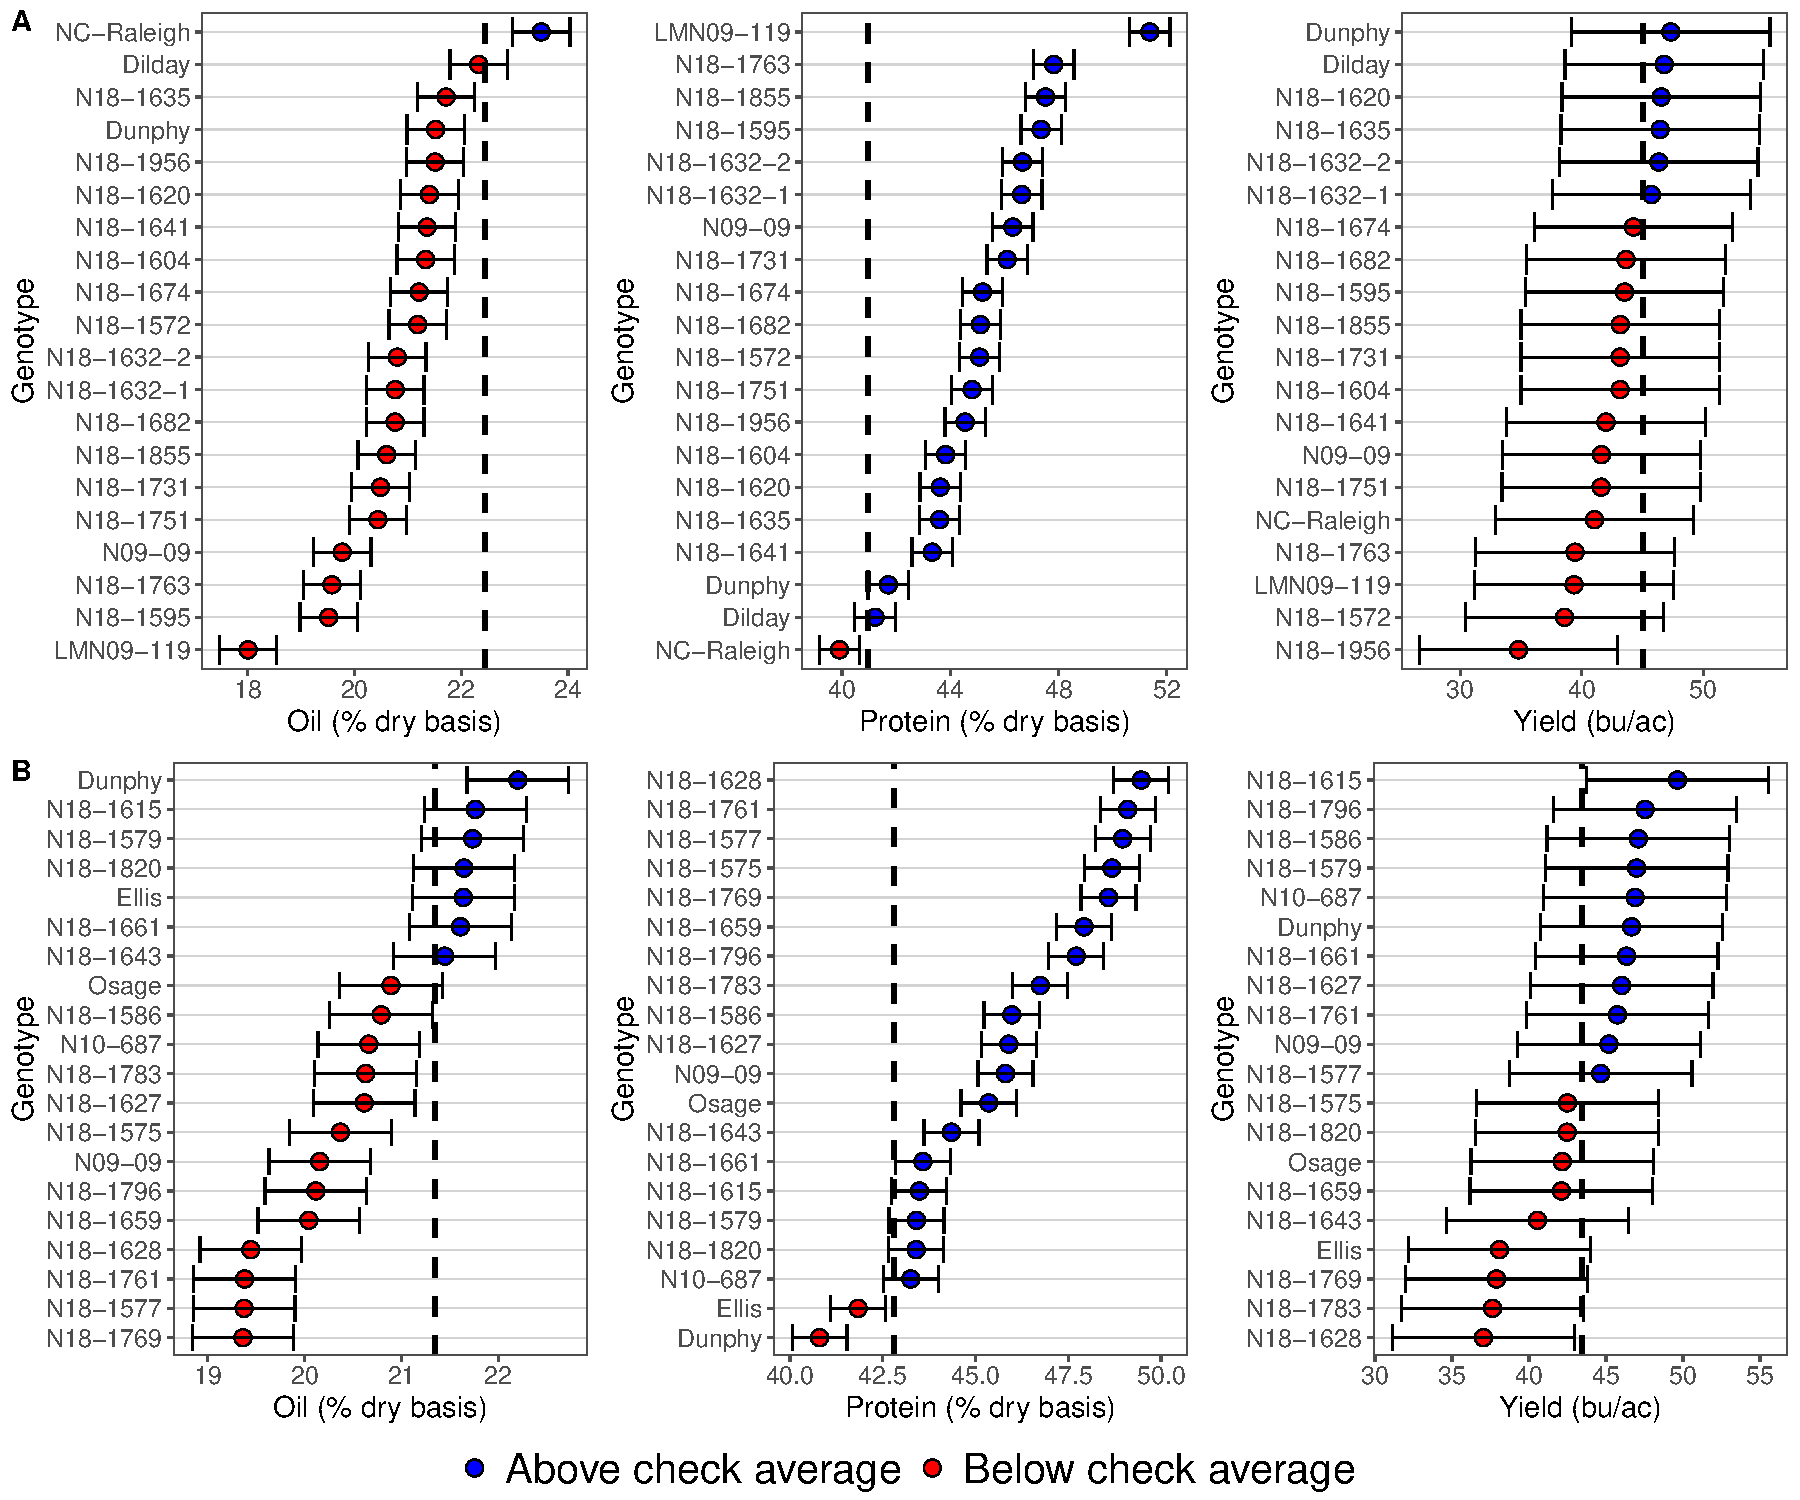
\includegraphics[width=15 cm]{C:/Users/Jay/Documents/R/Projects/Jay_yield/exports/plots/lsmean_scatterplot.pdf}
\caption{Genotype Least square means for seed oil, seed protein, and seed yield for soybean RILs in Test 1 (\textbf{A}) and Test 2 (\textbf{B}). Points indicate the least square means and error bars indicate the standard errors in the estimation of least square means. Blue dots indicate that a RIL has a least square mean above the average of the checks in the test and a color of red indicates that the RIL has a mean value below the check average. The check average is shown with the vertical dashed line.}
\end{figure}

\hypertarget{yield-contrasts}{%
\subsection{Yield contrasts}\label{yield-contrasts}}

Several RILs in each of the tests had yield that was comparable to that
of their check cultivars. This was determined both quantitatively
through the use of contrasts between the mean of each RIL with the
average of the yield check means, and qualitatively by inspecting the
standard errors on the estimation of the genotype marginal means for
yield. No genotypes had yield that was quantitatively higher than that
of the yield checks, however many had comparable yield. Many of these
genotypes with comparable yield also had protein content that was
superior to the check average in each test. No genotypes had oil that
was superior to the check cultivars, but some had comparable yield and
oil content as well as superior protein content.

RILs were also evaluated for lodging and seed quality. All RILs had seed
quality that was on par with that of the high-yielding checks however,
however 11 genotypes had lodging scores that were statistically
significantly greater than the checks on the basis of contrasts. These
RILs were removed from consideration for recommendation on the basis of
their relatively poor agronomic performance.

A detailed summary of all contrasts can be seen in supplementary table
1.

\hypertarget{genotypes-with-comparable-seed-yield-and-seed-oil-and-superior-seed-protein-content}{%
\subsection{Genotypes with comparable seed yield and seed oil and
superior seed protein
content}\label{genotypes-with-comparable-seed-yield-and-seed-oil-and-superior-seed-protein-content}}

Four genotypes had yield and oil that was similar to that of the yield
checks, and seed protein that was greater than the average of the
checks. These genotypes are N18-1635 from Test 1 and genotypes N18-1627,
N18-1643, and N18-1783 from Test 2. Summary data for these lines is
given in table 1.

\begin{table}[H]

\caption{Soybean genotypes with yield and seed oil comparable to check cultivars, and seed protein superior to check cultivars.}
\centering
\resizebox{\linewidth}{!}{
\begin{tabular}[t]{lllrlllrlllrll}
\toprule
\multicolumn{1}{c}{} & \multicolumn{1}{c}{} & \multicolumn{4}{c}{Protein} & \multicolumn{4}{c}{Yield} & \multicolumn{4}{c}{Oil} \\
\cmidrule(l{3pt}r{3pt}){3-6} \cmidrule(l{3pt}r{3pt}){7-10} \cmidrule(l{3pt}r{3pt}){11-14}
Genotype & Test Name & Value & Rank & Test Average & Check Average & Value & Rank & Test Average & Check Average & Value & Rank & Test Average & Check Average\\
\midrule
N18-1635 & Jay Test 1 & 43.61 (106.5\%) & 16 & 45.09 & 40.94 & 46.45 (103.1\%) & 4 & 42.92 & 45.05 & 21.72 (96.7\%) & 3 & 20.89 & 22.45\\
\cmidrule{1-14}
N18-1783 &  & 46.74 (109.3\%) & 8 &  &  & 37.63 (86.6\%) & 19 &  &  & 20.63 (96.5\%) & 11 &  & \\
\cmidrule{1-1}
\cmidrule{3-4}
\cmidrule{7-8}
\cmidrule{11-12}
N18-1627 &  & 45.9 (107.3\%) & 9 &  &  & 46.01 (105.9\%) & 8 &  &  & 20.62 (96.5\%) & 12 &  & \\
\cmidrule{1-1}
\cmidrule{3-4}
\cmidrule{7-8}
\cmidrule{11-12}
N18-1643 & \multirow{-3}{*}{\raggedright\arraybackslash Jay Test 2} & 44.35 (103.7\%) & 13 & \multirow{-3}{*}{\raggedright\arraybackslash 45.7} & \multirow{-3}{*}{\raggedright\arraybackslash 42.77} & 40.54 (93.3\%) & 16 & \multirow{-3}{*}{\raggedright\arraybackslash 43.65} & \multirow{-3}{*}{\raggedright\arraybackslash 43.44} & 21.45 (100.4\%) & 7 & \multirow{-3}{*}{\raggedright\arraybackslash 20.7} & \multirow{-3}{*}{\raggedright\arraybackslash 21.37}\\
\bottomrule
\multicolumn{14}{l}{\rule{0pt}{1em}\textsuperscript{*} The genotype name.}\\
\multicolumn{14}{l}{\rule{0pt}{1em}\textsuperscript{\dag} The genotype marginal mean for the phenotype (value divided by check average).}\\
\multicolumn{14}{l}{\rule{0pt}{1em}\textsuperscript{\ddag} The ranking of this genotype for the phenotype within its test.}\\
\multicolumn{14}{l}{\rule{0pt}{1em}\textsuperscript{\S} The average phenotype value for all genotypes in the test.}\\
\multicolumn{14}{l}{\rule{0pt}{1em}\textsuperscript{\P} The average value of the checks in the test.}\\
\end{tabular}}
\end{table}

A strong negative correlation was observed in both populations betweeen
seed oil and seed protein. This observation matches well with previous
findings on the inverse correlation between seed protein and seed oil.
Many RILs had high protein when compared with the check cultivars so it
was not surprising that relatively few had both a superior seed protein
content, and a comparable seed oil content.

\hypertarget{genotypes-with-comparable-yield-and-superior-protein}{%
\subsection{Genotypes with comparable yield and superior
protein}\label{genotypes-with-comparable-yield-and-superior-protein}}

Seventeen RILs had a similar yield and superior protein content to the
check cultivars. Summary data for the seed protein and seed yield of
these lines is given in table 2. The maximum yielding line

\begin{table}[H]

\caption{Soybean RILs with superior protein content and comparable yield performance to high-yielding check cultivars.}
\centering
\resizebox{\linewidth}{!}{
\begin{tabular}[t]{lllrlllrll}
\toprule
\multicolumn{1}{c}{} & \multicolumn{1}{c}{} & \multicolumn{4}{c}{Protein} & \multicolumn{4}{c}{Yield} \\
\cmidrule(l{3pt}r{3pt}){3-6} \cmidrule(l{3pt}r{3pt}){7-10}
Genotype & Test Name & Value & Rank & Test Average & Check Average & Value & Rank & Test Average & Check Average\\
\midrule
N18-1763 &  & 47.82 (116.8\%) & 2 &  &  & 39.45 (87.6\%) & 17 &  & \\
\cmidrule{1-1}
\cmidrule{3-4}
\cmidrule{7-8}
N18-1855 &  & 47.52 (116.1\%) & 3 &  &  & 43.17 (95.8\%) & 10 &  & \\
\cmidrule{1-1}
\cmidrule{3-4}
\cmidrule{7-8}
N18-1595 &  & 47.36 (115.7\%) & 4 &  &  & 43.52 (96.6\%) & 9 &  & \\
\cmidrule{1-1}
\cmidrule{3-4}
\cmidrule{7-8}
N18-1632-1 &  & 46.64 (113.9\%) & 6 &  &  & 45.73 (101.5\%) & 6 &  & \\
\cmidrule{1-1}
\cmidrule{3-4}
\cmidrule{7-8}
N18-1620 &  & 43.63 (106.6\%) & 15 &  &  & 46.54 (103.3\%) & 3 &  & \\
\cmidrule{1-1}
\cmidrule{3-4}
\cmidrule{7-8}
N18-1635 &  & 43.61 (106.5\%) & 16 &  &  & 46.45 (103.1\%) & 4 &  & \\
\cmidrule{1-1}
\cmidrule{3-4}
\cmidrule{7-8}
N18-1731 &  & 46.1 (112.6\%) & 8 &  &  & 43.16 (95.8\%) & 11 &  & \\
\cmidrule{1-1}
\cmidrule{3-4}
\cmidrule{7-8}
N18-1674 &  & 45.19 (110.4\%) & 9 &  &  & 44.26 (98.2\%) & 7 &  & \\
\cmidrule{1-1}
\cmidrule{3-4}
\cmidrule{7-8}
N18-1682 &  & 45.11 (110.2\%) & 10 &  &  & 43.64 (96.9\%) & 8 &  & \\
\cmidrule{1-1}
\cmidrule{3-4}
\cmidrule{7-8}
N18-1572 &  & 45.08 (110.1\%) & 11 &  &  & 38.58 (85.6\%) & 19 &  & \\
\cmidrule{1-1}
\cmidrule{3-4}
\cmidrule{7-8}
N18-1751 & \multirow{-11}{*}{\raggedright\arraybackslash Jay Test 1} & 44.8 (109.4\%) & 12 & \multirow{-11}{*}{\raggedright\arraybackslash 45.09} & \multirow{-11}{*}{\raggedright\arraybackslash 40.94} & 41.59 (92.3\%) & 15 & \multirow{-11}{*}{\raggedright\arraybackslash 42.92} & \multirow{-11}{*}{\raggedright\arraybackslash 45.05}\\
\cmidrule{1-10}
N18-1761 &  & 49.1 (114.8\%) & 2 &  &  & 45.74 (105.3\%) & 9 &  & \\
\cmidrule{1-1}
\cmidrule{3-4}
\cmidrule{7-8}
N18-1575 &  & 48.67 (113.8\%) & 4 &  &  & 42.49 (97.8\%) & 12 &  & \\
\cmidrule{1-1}
\cmidrule{3-4}
\cmidrule{7-8}
N18-1769 &  & 48.58 (113.6\%) & 5 &  &  & 37.88 (87.2\%) & 18 &  & \\
\cmidrule{1-1}
\cmidrule{3-4}
\cmidrule{7-8}
N18-1783 &  & 46.74 (109.3\%) & 8 &  &  & 37.63 (86.6\%) & 19 &  & \\
\cmidrule{1-1}
\cmidrule{3-4}
\cmidrule{7-8}
N18-1627 &  & 45.9 (107.3\%) & 9 &  &  & 46.01 (105.9\%) & 8 &  & \\
\cmidrule{1-1}
\cmidrule{3-4}
\cmidrule{7-8}
N18-1643 & \multirow{-6}{*}{\raggedright\arraybackslash Jay Test 2} & 44.35 (103.7\%) & 13 & \multirow{-6}{*}{\raggedright\arraybackslash 45.7} & \multirow{-6}{*}{\raggedright\arraybackslash 42.77} & 40.54 (93.3\%) & 16 & \multirow{-6}{*}{\raggedright\arraybackslash 43.65} & \multirow{-6}{*}{\raggedright\arraybackslash 43.44}\\
\bottomrule
\multicolumn{10}{l}{\rule{0pt}{1em}\textsuperscript{*} The genotype name.}\\
\multicolumn{10}{l}{\rule{0pt}{1em}\textsuperscript{\dag} The genotype marginal mean for the phenotype (value divided by check average).}\\
\multicolumn{10}{l}{\rule{0pt}{1em}\textsuperscript{\ddag} The ranking of this genotype for the phenotype within its test.}\\
\multicolumn{10}{l}{\rule{0pt}{1em}\textsuperscript{\S} The average phenotype value for all genotypes in the test.}\\
\multicolumn{10}{l}{\rule{0pt}{1em}\textsuperscript{\P} The average value of the checks in the test.}\\
\end{tabular}}
\end{table}

Among these genotypes are several with both average seed protein and
average seed yield that were greater than the averages of the checks for
each test. These N18-1632-1, N18-1620, N18-1635 from test 1 and RILs
N18-1761 and N18-1627 from test 2. Of particular note are genotypes
N18-1632-1 from test 1 and N18-1761 from test 2. On average, genotype
N18-1632-1 had a protein content that was 113.9\% of the check average
while maintaining a yield average that was 101.5\% that of the check
average.

\hypertarget{conclusion}{%
\section{Conclusion}\label{conclusion}}

We have identified several genotypes with seed yield that is comparable
to existing cultivars that are commonly used in production. Many of
these genotypes have seed protein content that exceeds that of the check
cultivars, and some of these with superior protein have a seed oil
content that is comparable to these check cultivars as well. These
genotypes have good agronomic qualities as well and will provide both
breeders and growers with new options for genotypes that can be used in
production or used in breeding programs that seek to improve valuable
soybean seed composition traits.

% %%%%%%%%%%%%%%%%%%%%%%%%%%%%%%%%%%%%%%%%%%
% %% optional
% \supplementary{The following are available online at www.mdpi.com/link, Figure S1: title, Table S1: title, Video S1: title.}
%
% % Only for the journal Methods and Protocols:
% % If you wish to submit a video article, please do so with any other supplementary material.
% % \supplementary{The following are available at www.mdpi.com/link: Figure S1: title, Table S1: title, Video S1: title. A supporting video article is available at doi: link.}

\vspace{6pt}

%%%%%%%%%%%%%%%%%%%%%%%%%%%%%%%%%%%%%%%%%%
\acknowledgments{All sources of funding of the study should be
disclosed. Please clearly indicate grants that you have received in
support of your research work. Clearly state if you received funds for
covering the costs to publish in open access.}

%%%%%%%%%%%%%%%%%%%%%%%%%%%%%%%%%%%%%%%%%%
\authorcontributions{For research articles with several authors, a short
paragraph specifying their individual contributions must be provided.
The following statements should be used ``X.X. and Y.Y. conceive and
designed the experiments; X.X. performed the experiments; X.X. and Y.Y.
analyzed the data; W.W. contributed reagents/materials/analysis tools;
Y.Y. wrote the paper.'\,' Authorship must be limited to those who have
contributed substantially to the work reported.}

%%%%%%%%%%%%%%%%%%%%%%%%%%%%%%%%%%%%%%%%%%
\conflictsofinterest{The authors declare no conflict of interest.}

%%%%%%%%%%%%%%%%%%%%%%%%%%%%%%%%%%%%%%%%%%
%% optional
\abbreviations{The following abbreviations are used in this manuscript:\\

\noindent
\begin{tabular}{@{}ll}
RIL & Recombinant inbred line \\
RCBD & Randomized complete block design \\
CLA & Central crops research station \\
CAS & Caswell research farm \\
PLY & Tidewater research station \\
\end{tabular}}

\input{"appendix.tex"}

%%%%%%%%%%%%%%%%%%%%%%%%%%%%%%%%%%%%%%%%%%
% Citations and References in Supplementary files are permitted provided that they also appear in the reference list here.

%=====================================
% References, variant A: internal bibliography
%=====================================
%\reftitle{References}
%\begin{thebibliography}{999}
% Reference 1
%\bibitem[Author1(year)]{ref-journal}
%Author1, T. The title of the cited article. {\em Journal Abbreviation} {\bf 2008}, {\em 10}, 142--149.
% Reference 2
%\bibitem[Author2(year)]{ref-book}
%Author2, L. The title of the cited contribution. In {\em The Book Title}; Editor1, F., Editor2, A., Eds.; Publishing House: City, Country, 2007; pp. 32--58.
%\end{thebibliography}

% The following MDPI journals use author-date citation: Arts, Econometrics, Economies, Genealogy, Humanities, IJFS, JRFM, Laws, Religions, Risks, Social Sciences. For those journals, please follow the formatting guidelines on http://www.mdpi.com/authors/references
% To cite two works by the same author: \citeauthor{ref-journal-1a} (\citeyear{ref-journal-1a}, \citeyear{ref-journal-1b}). This produces: Whittaker (1967, 1975)
% To cite two works by the same author with specific pages: \citeauthor{ref-journal-3a} (\citeyear{ref-journal-3a}, p. 328; \citeyear{ref-journal-3b}, p.475). This produces: Wong (1999, p. 328; 2000, p. 475)

%=====================================
% References, variant B: external bibliography
%=====================================
\reftitle{References}
\externalbibliography{yes}
\bibliography{mybibfile.bib}

%%%%%%%%%%%%%%%%%%%%%%%%%%%%%%%%%%%%%%%%%%
%% optional
\sampleavailability{Samples of the compounds \ldots\ldots{} are
available from the authors.}

%% for journal Sci
%\reviewreports{\\
%Reviewer 1 comments and authors’ response\\
%Reviewer 2 comments and authors’ response\\
%Reviewer 3 comments and authors’ response
%}

%%%%%%%%%%%%%%%%%%%%%%%%%%%%%%%%%%%%%%%%%%


\end{document}
